\begin{figure}
  \setlength{\unitlength}{\textwidth}
\fbox{
  \begin{picture}(1,0.7)(0,0.5)
    
    % % %90
      \put(0,0.9){\includegraphics[width=0.5\unitlength]{../FnP/gnuplot/fsi_displacement.eps}}
      \put(0.495,0.9){\includegraphics[width=0.5\unitlength]{../FnP/gnuplot/fsi_velocity.eps}}
      \put(0.25,0.6){\includegraphics[width=0.5\unitlength]{../FnP/gnuplot/fsi_power.eps}}
     
   
	
            
      
      
   
 	\put(0,1.02){ $\frac{A}{D}$} 	
 	\put(0.495,1.02){ $\frac{V}{D}$}
 	\put(0.2,0.75){ $\frac{P_{m}}{\rho \mathcal{A}U^3 }$}
 	
 	 	\put(0.25,0.88){ \ustar} 	
 	 	\put(0.8,0.88){ \ustar}
 	 	\put(0.5,0.58){ \ustar}



    \put(0.07,1.1){(a)}
    \put(0.575,1.1){(b)}
    \put(0.31,0.8){(c)}
   
       

  \end{picture}
}  
  \caption{Comparison of QSS (\ding{83}) and FSI (\ding{108}) data of displacement amplitude, velocity amplitude and mean power as a function of \ustar represented by (a), (b) and (c)respectively. Data were obtained at Re=165 and $\zeta=0.075$. An average error of $34\%$ could be observed for both displacement and velocity amplitude. Essential physics i.e the rise and fall of mean power could be captured of the FSI data}
    \label{fig:FSI_QSS_compare}
\end{figure}